\documentclass[border=0pt]{standalone}
\usepackage{iftex}
\ifPDFTeX
  \usepackage[T1]{fontenc}
  \usepackage{DejaVuSans}
  \renewcommand*\familydefault{\sfdefault}
  \usepackage[italic]{mathastext}
\else
  \usepackage{unicode-math}
  \setmainfont{DejaVuSans.ttf}[BoldFont=DejaVuSans-Bold.ttf,ItalicFont=DejaVuSans-Oblique.ttf,
    BoldItalicFont=DejaVuSans-BoldOblique.ttf]
  \setmathfont{texgyredejavu-math.otf}
\fi
\ifPDFTeX  % one glyph of matplotlib mathtext, by Unicode code point (hex)
  \def\mplchar#1{\ifnum"#1="2212 \ensuremath{-}\else\ifnum"#1="D7 \texttimes\else\char"#1\relax\fi\fi}
\else
  \def\mplchar#1{\char"#1\relax}
\fi
\frenchspacing  % matplotlib puts a normal space after punctuation
\usepackage{pgfplots}
\pgfplotsset{compat=1.18}
% matplotlib marker shapes; \pgfplotmarksize = half the matplotlib marker size
\pgfdeclareplotmark{mpl-o}{\pgfpathcircle{\pgfpointorigin}{\pgfplotmarksize}\pgfusepathqfillstroke}
\pgfdeclareplotmark{mpl-o-open}{\pgfpathcircle{\pgfpointorigin}{\pgfplotmarksize}\pgfusepathqstroke}
\pgfdeclareplotmark{mpl-s}{\pgfpathrectangle{\pgfpoint{-\pgfplotmarksize}{-\pgfplotmarksize}}{\pgfpoint{2\pgfplotmarksize}{2\pgfplotmarksize}}\pgfusepathqfillstroke}
\pgfdeclareplotmark{mpl-s-open}{\pgfpathrectangle{\pgfpoint{-\pgfplotmarksize}{-\pgfplotmarksize}}{\pgfpoint{2\pgfplotmarksize}{2\pgfplotmarksize}}\pgfusepathqstroke}
\def\mpltriangle#1{\pgfpathmoveto{\pgfpoint{0pt}{#1\pgfplotmarksize}}\pgfpathlineto{\pgfpoint{-\pgfplotmarksize}{-#1\pgfplotmarksize}}\pgfpathlineto{\pgfpoint{\pgfplotmarksize}{-#1\pgfplotmarksize}}\pgfpathclose}
\pgfdeclareplotmark{mpl-^}{\mpltriangle{}\pgfusepathqfillstroke}
\pgfdeclareplotmark{mpl-^-open}{\mpltriangle{}\pgfusepathqstroke}
\pgfdeclareplotmark{mpl-v}{\mpltriangle{-}\pgfusepathqfillstroke}
\pgfdeclareplotmark{mpl-v-open}{\mpltriangle{-}\pgfusepathqstroke}
\def\mpldiamond{\pgfpathmoveto{\pgfpoint{0pt}{1.41421\pgfplotmarksize}}\pgfpathlineto{\pgfpoint{-1.41421\pgfplotmarksize}{0pt}}\pgfpathlineto{\pgfpoint{0pt}{-1.41421\pgfplotmarksize}}\pgfpathlineto{\pgfpoint{1.41421\pgfplotmarksize}{0pt}}\pgfpathclose}
\pgfdeclareplotmark{mpl-D}{\mpldiamond\pgfusepathqfillstroke}
\pgfdeclareplotmark{mpl-D-open}{\mpldiamond\pgfusepathqstroke}
\pgfdeclareplotmark{mpl-x}{\pgfpathmoveto{\pgfpoint{-\pgfplotmarksize}{-\pgfplotmarksize}}\pgfpathlineto{\pgfpoint{\pgfplotmarksize}{\pgfplotmarksize}}\pgfpathmoveto{\pgfpoint{-\pgfplotmarksize}{\pgfplotmarksize}}\pgfpathlineto{\pgfpoint{\pgfplotmarksize}{-\pgfplotmarksize}}\pgfsetbuttcap\pgfusepathqstroke}
\pgfdeclareplotmark{mpl-+}{\pgfpathmoveto{\pgfpoint{-\pgfplotmarksize}{0pt}}\pgfpathlineto{\pgfpoint{\pgfplotmarksize}{0pt}}\pgfpathmoveto{\pgfpoint{0pt}{-\pgfplotmarksize}}\pgfpathlineto{\pgfpoint{0pt}{\pgfplotmarksize}}\pgfsetbuttcap\pgfusepathqstroke}
\def\mplplus{\pgfpathmoveto{\pgfpoint{-0.33333\pgfplotmarksize}{-\pgfplotmarksize}}\pgfpathlineto{\pgfpoint{0.33333\pgfplotmarksize}{-\pgfplotmarksize}}\pgfpathlineto{\pgfpoint{0.33333\pgfplotmarksize}{-0.33333\pgfplotmarksize}}\pgfpathlineto{\pgfpoint{\pgfplotmarksize}{-0.33333\pgfplotmarksize}}\pgfpathlineto{\pgfpoint{\pgfplotmarksize}{0.33333\pgfplotmarksize}}\pgfpathlineto{\pgfpoint{0.33333\pgfplotmarksize}{0.33333\pgfplotmarksize}}\pgfpathlineto{\pgfpoint{0.33333\pgfplotmarksize}{\pgfplotmarksize}}\pgfpathlineto{\pgfpoint{-0.33333\pgfplotmarksize}{\pgfplotmarksize}}\pgfpathlineto{\pgfpoint{-0.33333\pgfplotmarksize}{0.33333\pgfplotmarksize}}\pgfpathlineto{\pgfpoint{-\pgfplotmarksize}{0.33333\pgfplotmarksize}}\pgfpathlineto{\pgfpoint{-\pgfplotmarksize}{-0.33333\pgfplotmarksize}}\pgfpathlineto{\pgfpoint{-0.33333\pgfplotmarksize}{-0.33333\pgfplotmarksize}}\pgfpathclose}
\pgfdeclareplotmark{mpl-P}{\mplplus\pgfusepathqfillstroke}
\pgfdeclareplotmark{mpl-P-open}{\mplplus\pgfusepathqstroke}
\def\mplstar{\pgfpathmoveto{\pgfpointpolar{90}{\pgfplotmarksize}}%
  \foreach \i in {1,...,4} {\pgfpathlineto{\pgfpointpolar{90+72*\i-36}{0.381966\pgfplotmarksize}}\pgfpathlineto{\pgfpointpolar{90+72*\i}{\pgfplotmarksize}}}%
  \pgfpathlineto{\pgfpointpolar{54}{0.381966\pgfplotmarksize}}\pgfpathclose}
\pgfdeclareplotmark{mpl-*}{\mplstar\pgfusepathqfillstroke}
\pgfdeclareplotmark{mpl-*-open}{\mplstar\pgfusepathqstroke}
\def\mpltriside#1{\pgfpathmoveto{\pgfpoint{#1\pgfplotmarksize}{0pt}}\pgfpathlineto{\pgfpoint{-#1\pgfplotmarksize}{\pgfplotmarksize}}\pgfpathlineto{\pgfpoint{-#1\pgfplotmarksize}{-\pgfplotmarksize}}\pgfpathclose}
\pgfdeclareplotmark{mpl-<}{\mpltriside{-}\pgfusepathqfillstroke}
\pgfdeclareplotmark{mpl-<-open}{\mpltriside{-}\pgfusepathqstroke}
\pgfdeclareplotmark{mpl->}{\mpltriside{}\pgfusepathqfillstroke}
\pgfdeclareplotmark{mpl->-open}{\mpltriside{}\pgfusepathqstroke}
\def\mplpolygon#1{\pgfpathmoveto{\pgfpointpolar{90}{\pgfplotmarksize}}\foreach \i in {1,...,#1} {\pgfpathlineto{\pgfpointpolar{90+360/#1*\i}{\pgfplotmarksize}}}\pgfpathclose}
\pgfdeclareplotmark{mpl-p}{\mplpolygon{5}\pgfusepathqfillstroke}
\pgfdeclareplotmark{mpl-p-open}{\mplpolygon{5}\pgfusepathqstroke}
\pgfdeclareplotmark{mpl-h}{\mplpolygon{6}\pgfusepathqfillstroke}
\pgfdeclareplotmark{mpl-h-open}{\mplpolygon{6}\pgfusepathqstroke}
\definecolor{mplc0}{HTML}{B0B0B0}
\definecolor{mplc1}{HTML}{000000}
\definecolor{mplc2}{HTML}{1F77B4}
\definecolor{mplc3}{HTML}{D62728}
\definecolor{mplc4}{HTML}{DAA520}
\definecolor{mplc5}{HTML}{9467BD}
\definecolor{mplc6}{HTML}{17BECF}
\definecolor{mplc7}{HTML}{2CA02C}
\begin{document}
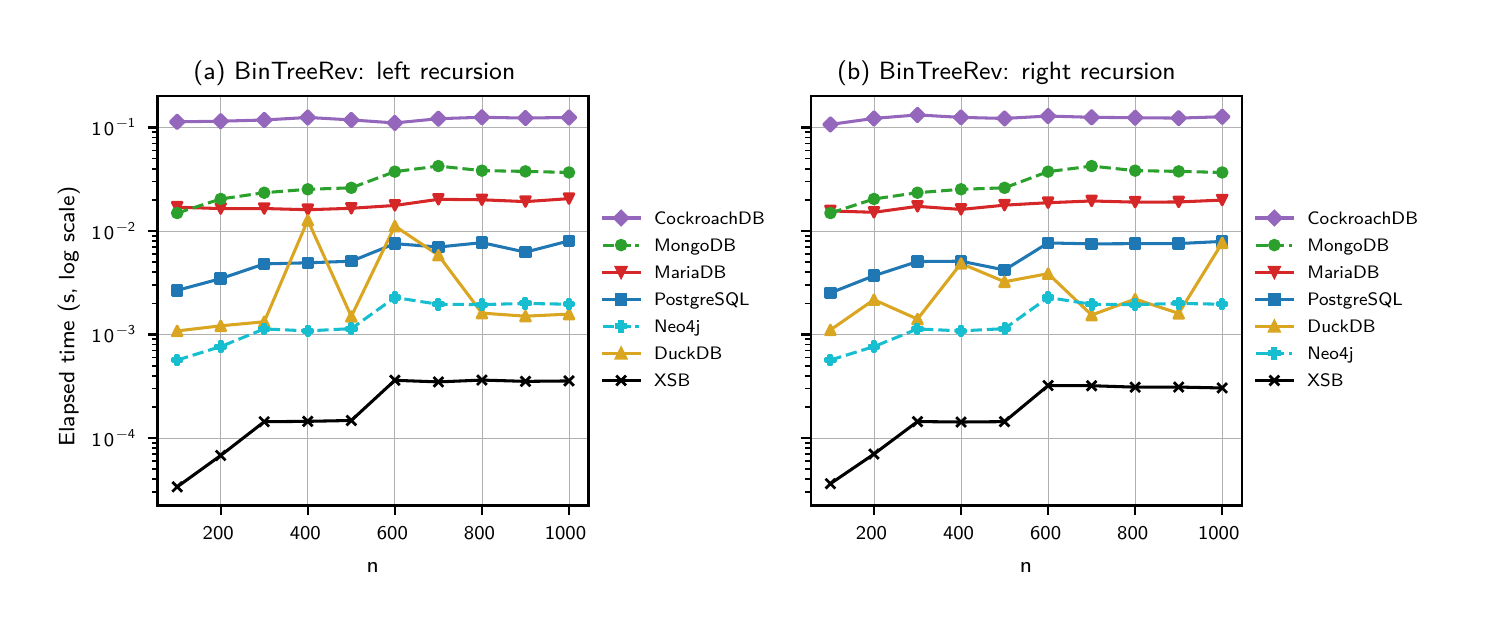
\begin{tikzpicture}
\useasboundingbox (0in,0in) rectangle (7.2in,2.9in);
\begin{axis}[at={(0.6495in,0.5111in)}, anchor=south west, scale only axis, width=2.1552in, height=2.0456in, xmin=55, xmax=1045, ymin=2.232350325e-05, ymax=0.1999237199, enlargelimits=false, clip=true, axis on top=false, axis line style={line width=0.8bp, black}, tick align=outside, tick pos=left, major tick length=3.5bp, minor tick length=2bp, major tick style={line width=0.8bp, black}, minor tick style={line width=0.6bp, black}, xticklabels={}, yticklabels={}, scaled x ticks=false, scaled y ticks=false, xlabel={}, ylabel={}, title={}, xtick={200,400,600,800,1000}, minor xtick={}, ymode=log, log basis y=10, ytick={0.0001,0.001,0.01,0.1}, minor ytick={3e-05,4e-05,5e-05,6e-05,7e-05,8e-05,9e-05,0.0002,0.0003,0.0004,0.0005,0.0006,0.0007,0.0008,0.0009,0.002,0.003,0.004,0.005,0.006,0.007,0.008,0.009,0.02,0.03,0.04,0.05,0.06,0.07,0.08,0.09}, xmajorgrids, ymajorgrids, major grid style={line width=0.3bp, draw=mplc0}]
\addplot[color=mplc1, line width=1.1bp, line join=round, solid, line cap=rect, mark=mpl-x, mark size=1.75bp, mark options={solid, line width=1bp, draw=mplc1}] coordinates {(100,3.37600708e-05) (200,6.785392761e-05) (300,0.0001437664032) (400,0.0001450061798) (500,0.000147819519) (600,0.0003612041473) (700,0.0003486156464) (800,0.000363111496) (900,0.0003528594971) (1000,0.0003561496735)};
\addplot[color=mplc2, line width=1.1bp, line join=round, solid, line cap=rect, mark=mpl-s, mark size=1.75bp, mark options={solid, line width=1bp, draw=mplc2, fill=mplc2}] coordinates {(100,0.002672891784) (200,0.003464066808) (300,0.004809175199) (400,0.004930441396) (500,0.005105791602) (600,0.007546508394) (700,0.007001341798) (800,0.007718774804) (900,0.006250766804) (1000,0.008025483415)};
\addplot[color=mplc3, line width=1.1bp, line join=round, solid, line cap=rect, mark=mpl-v, mark size=1.75bp, mark options={solid, line width=1bp, draw=mplc3, fill=mplc3}] coordinates {(100,0.01699153379) (200,0.01646330821) (300,0.0164876668) (400,0.0160483584) (500,0.01657235839) (600,0.01764689161) (700,0.02023165821) (800,0.02002529161) (900,0.01923004161) (1000,0.02053638338)};
\addplot[color=mplc4, line width=1.1bp, line join=round, solid, line cap=rect, mark=mpl-^, mark size=1.75bp, mark options={solid, line width=1bp, draw=mplc4, fill=mplc4}] coordinates {(100,0.00108344981) (200,0.001213675202) (300,0.001328708197) (400,0.012698525) (500,0.001495500002) (600,0.01116557479) (700,0.005838741804) (800,0.001609508391) (900,0.0015040586) (1000,0.001574483002)};
\addplot[color=mplc5, line width=1.1bp, line join=round, solid, line cap=rect, mark=mpl-D, mark size=1.75bp, mark options={solid, line width=1bp, draw=mplc5, fill=mplc5}] coordinates {(100,0.113380225) (200,0.1149991502) (300,0.1181352666) (400,0.124986325) (500,0.1183181334) (600,0.1106061336) (700,0.1215974082) (800,0.1254772418) (900,0.1232514752) (1000,0.1250653166)};
\addplot[color=mplc6, line width=1.1bp, line join=round, dash pattern=on 4.07bp off 1.76bp, line cap=butt, mark=mpl-P, mark size=1.75bp, mark options={solid, line width=1bp, draw=mplc6, fill=mplc6}] coordinates {(100,0.0005662665819) (200,0.000764808408) (300,0.001132675004) (400,0.001084500004) (500,0.001139641798) (600,0.002278350003) (700,0.001959858218) (800,0.001946774998) (900,0.001996633213) (1000,0.00196210799)};
\addplot[color=mplc7, line width=1.1bp, line join=round, dash pattern=on 4.07bp off 1.76bp, line cap=butt, mark=mpl-o, mark size=1.75bp, mark options={solid, line width=1bp, draw=mplc7, fill=mplc7}] coordinates {(100,0.01490103321) (200,0.0203909914) (300,0.02343996661) (400,0.02528171662) (500,0.02612852481) (600,0.03744473341) (700,0.04237827499) (800,0.0382853998) (900,0.0376632918) (1000,0.03678338339)};
\end{axis}
\begin{axis}[at={(3.9157in,0.5111in)}, anchor=south west, scale only axis, width=2.1552in, height=2.0456in, xmin=55, xmax=1045, ymin=2.232350325e-05, ymax=0.1999237199, enlargelimits=false, clip=true, axis on top=false, axis line style={line width=0.8bp, black}, tick align=outside, tick pos=left, major tick length=3.5bp, minor tick length=2bp, major tick style={line width=0.8bp, black}, minor tick style={line width=0.6bp, black}, xticklabels={}, yticklabels={}, scaled x ticks=false, scaled y ticks=false, xlabel={}, ylabel={}, title={}, xtick={200,400,600,800,1000}, minor xtick={}, ymode=log, log basis y=10, ytick={0.0001,0.001,0.01,0.1}, minor ytick={3e-05,4e-05,5e-05,6e-05,7e-05,8e-05,9e-05,0.0002,0.0003,0.0004,0.0005,0.0006,0.0007,0.0008,0.0009,0.002,0.003,0.004,0.005,0.006,0.007,0.008,0.009,0.02,0.03,0.04,0.05,0.06,0.07,0.08,0.09}, xmajorgrids, ymajorgrids, major grid style={line width=0.3bp, draw=mplc0}]
\addplot[color=mplc1, line width=1.1bp, line join=round, solid, line cap=rect, mark=mpl-x, mark size=1.75bp, mark options={solid, line width=1bp, draw=mplc1}] coordinates {(100,3.623962402e-05) (200,6.999969482e-05) (300,0.0001442909241) (400,0.0001428127289) (500,0.0001440048218) (600,0.0003213882446) (700,0.000320148468) (800,0.0003102302551) (900,0.0003108501434) (1000,0.0003045558929)};
\addplot[color=mplc2, line width=1.1bp, line join=round, solid, line cap=rect, mark=mpl-s, mark size=1.75bp, mark options={solid, line width=1bp, draw=mplc2, fill=mplc2}] coordinates {(100,0.002522508602) (200,0.003697083401) (300,0.005069041613) (400,0.005107458401) (500,0.004202958383) (600,0.00766964982) (700,0.007509150216) (800,0.007546275191) (900,0.007566391374) (1000,0.007931916381)};
\addplot[color=mplc3, line width=1.1bp, line join=round, solid, line cap=rect, mark=mpl-v, mark size=1.75bp, mark options={solid, line width=1bp, draw=mplc3, fill=mplc3}] coordinates {(100,0.01563245) (200,0.01515125019) (300,0.01730340018) (400,0.01615358342) (500,0.01777036696) (600,0.01876033299) (700,0.01950392521) (800,0.01899947461) (900,0.01906782499) (1000,0.01990670861)};
\addplot[color=mplc4, line width=1.1bp, line join=round, solid, line cap=rect, mark=mpl-^, mark size=1.75bp, mark options={solid, line width=1bp, draw=mplc4, fill=mplc4}] coordinates {(100,0.001106791594) (200,0.002169866813) (300,0.001408791402) (400,0.004857625405) (500,0.003232849995) (600,0.003875033208) (700,0.001542949979) (800,0.00219866659) (900,0.001600950211) (1000,0.007692775212)};
\addplot[color=mplc5, line width=1.1bp, line join=round, solid, line cap=rect, mark=mpl-D, mark size=1.75bp, mark options={solid, line width=1bp, draw=mplc5, fill=mplc5}] coordinates {(100,0.107003775) (200,0.1223842252) (300,0.1321975252) (400,0.1251800668) (500,0.1222521498) (600,0.1290243334) (700,0.1253713918) (800,0.1242494918) (900,0.123176775) (1000,0.1269378998)};
\addplot[color=mplc6, line width=1.1bp, line join=round, dash pattern=on 4.07bp off 1.76bp, line cap=butt, mark=mpl-P, mark size=1.75bp, mark options={solid, line width=1bp, draw=mplc6, fill=mplc6}] coordinates {(100,0.0005662665819) (200,0.000764808408) (300,0.001132675004) (400,0.001084500004) (500,0.001139641798) (600,0.002278350003) (700,0.001959858218) (800,0.001946774998) (900,0.001996633213) (1000,0.00196210799)};
\addplot[color=mplc7, line width=1.1bp, line join=round, dash pattern=on 4.07bp off 1.76bp, line cap=butt, mark=mpl-o, mark size=1.75bp, mark options={solid, line width=1bp, draw=mplc7, fill=mplc7}] coordinates {(100,0.01490103321) (200,0.0203909914) (300,0.02343996661) (400,0.02528171662) (500,0.02612852481) (600,0.03744473341) (700,0.04237827499) (800,0.0382853998) (900,0.0376632918) (1000,0.03678338339)};
\end{axis}
\draw[color=mplc5, line width=1.1bp, line join=round, solid, line cap=rect] (2.8769in,1.9483in) -- (3.0575in,1.9483in);
\begin{scope}[solid, line width=1bp, draw=mplc5, fill=mplc5]\pgftransformshift{\pgfpoint{2.9672in}{1.9483in}}\pgfsetplotmarksize{1.75bp}\pgfuseplotmark{mpl-D}\end{scope}
\draw[color=mplc7, line width=1.1bp, line join=round, dash pattern=on 4.07bp off 1.76bp, line cap=butt] (2.8769in,1.8129in) -- (3.0575in,1.8129in);
\begin{scope}[solid, line width=1bp, draw=mplc7, fill=mplc7]\pgftransformshift{\pgfpoint{2.9672in}{1.8129in}}\pgfsetplotmarksize{1.75bp}\pgfuseplotmark{mpl-o}\end{scope}
\draw[color=mplc3, line width=1.1bp, line join=round, solid, line cap=rect] (2.8769in,1.6775in) -- (3.0575in,1.6775in);
\begin{scope}[solid, line width=1bp, draw=mplc3, fill=mplc3]\pgftransformshift{\pgfpoint{2.9672in}{1.6775in}}\pgfsetplotmarksize{1.75bp}\pgfuseplotmark{mpl-v}\end{scope}
\draw[color=mplc2, line width=1.1bp, line join=round, solid, line cap=rect] (2.8769in,1.542in) -- (3.0575in,1.542in);
\begin{scope}[solid, line width=1bp, draw=mplc2, fill=mplc2]\pgftransformshift{\pgfpoint{2.9672in}{1.542in}}\pgfsetplotmarksize{1.75bp}\pgfuseplotmark{mpl-s}\end{scope}
\draw[color=mplc6, line width=1.1bp, line join=round, dash pattern=on 4.07bp off 1.76bp, line cap=butt] (2.8769in,1.4066in) -- (3.0575in,1.4066in);
\begin{scope}[solid, line width=1bp, draw=mplc6, fill=mplc6]\pgftransformshift{\pgfpoint{2.9672in}{1.4066in}}\pgfsetplotmarksize{1.75bp}\pgfuseplotmark{mpl-P}\end{scope}
\draw[color=mplc4, line width=1.1bp, line join=round, solid, line cap=rect] (2.8769in,1.2712in) -- (3.0575in,1.2712in);
\begin{scope}[solid, line width=1bp, draw=mplc4, fill=mplc4]\pgftransformshift{\pgfpoint{2.9672in}{1.2712in}}\pgfsetplotmarksize{1.75bp}\pgfuseplotmark{mpl-^}\end{scope}
\draw[color=mplc1, line width=1.1bp, line join=round, solid, line cap=rect] (2.8769in,1.1358in) -- (3.0575in,1.1358in);
\begin{scope}[solid, line width=1bp, draw=mplc1]\pgftransformshift{\pgfpoint{2.9672in}{1.1358in}}\pgfsetplotmarksize{1.75bp}\pgfuseplotmark{mpl-x}\end{scope}
\draw[color=mplc5, line width=1.1bp, line join=round, solid, line cap=rect] (6.1431in,1.9483in) -- (6.3237in,1.9483in);
\begin{scope}[solid, line width=1bp, draw=mplc5, fill=mplc5]\pgftransformshift{\pgfpoint{6.2334in}{1.9483in}}\pgfsetplotmarksize{1.75bp}\pgfuseplotmark{mpl-D}\end{scope}
\draw[color=mplc7, line width=1.1bp, line join=round, dash pattern=on 4.07bp off 1.76bp, line cap=butt] (6.1431in,1.8129in) -- (6.3237in,1.8129in);
\begin{scope}[solid, line width=1bp, draw=mplc7, fill=mplc7]\pgftransformshift{\pgfpoint{6.2334in}{1.8129in}}\pgfsetplotmarksize{1.75bp}\pgfuseplotmark{mpl-o}\end{scope}
\draw[color=mplc3, line width=1.1bp, line join=round, solid, line cap=rect] (6.1431in,1.6775in) -- (6.3237in,1.6775in);
\begin{scope}[solid, line width=1bp, draw=mplc3, fill=mplc3]\pgftransformshift{\pgfpoint{6.2334in}{1.6775in}}\pgfsetplotmarksize{1.75bp}\pgfuseplotmark{mpl-v}\end{scope}
\draw[color=mplc2, line width=1.1bp, line join=round, solid, line cap=rect] (6.1431in,1.542in) -- (6.3237in,1.542in);
\begin{scope}[solid, line width=1bp, draw=mplc2, fill=mplc2]\pgftransformshift{\pgfpoint{6.2334in}{1.542in}}\pgfsetplotmarksize{1.75bp}\pgfuseplotmark{mpl-s}\end{scope}
\draw[color=mplc4, line width=1.1bp, line join=round, solid, line cap=rect] (6.1431in,1.4066in) -- (6.3237in,1.4066in);
\begin{scope}[solid, line width=1bp, draw=mplc4, fill=mplc4]\pgftransformshift{\pgfpoint{6.2334in}{1.4066in}}\pgfsetplotmarksize{1.75bp}\pgfuseplotmark{mpl-^}\end{scope}
\draw[color=mplc6, line width=1.1bp, line join=round, dash pattern=on 4.07bp off 1.76bp, line cap=butt] (6.1431in,1.2712in) -- (6.3237in,1.2712in);
\begin{scope}[solid, line width=1bp, draw=mplc6, fill=mplc6]\pgftransformshift{\pgfpoint{6.2334in}{1.2712in}}\pgfsetplotmarksize{1.75bp}\pgfuseplotmark{mpl-P}\end{scope}
\draw[color=mplc1, line width=1.1bp, line join=round, solid, line cap=rect] (6.1431in,1.1358in) -- (6.3237in,1.1358in);
\begin{scope}[solid, line width=1bp, draw=mplc1]\pgftransformshift{\pgfpoint{6.2334in}{1.1358in}}\pgfsetplotmarksize{1.75bp}\pgfuseplotmark{mpl-x}\end{scope}
\node[anchor=base west, inner sep=0pt, text=mplc1, font=\fontsize{7bp}{8.4bp}\selectfont] at (0.8724in,0.34in) {200};
\node[anchor=base west, inner sep=0pt, text=mplc1, font=\fontsize{7bp}{8.4bp}\selectfont] at (1.3078in,0.34in) {400};
\node[anchor=base west, inner sep=0pt, text=mplc1, font=\fontsize{7bp}{8.4bp}\selectfont] at (1.7432in,0.34in) {600};
\node[anchor=base west, inner sep=0pt, text=mplc1, font=\fontsize{7bp}{8.4bp}\selectfont] at (2.1785in,0.34in) {800};
\node[anchor=base west, inner sep=0pt, text=mplc1, font=\fontsize{7bp}{8.4bp}\selectfont] at (2.583in,0.34in) {1000};
\node[anchor=base west, inner sep=0pt, text=mplc1, font=\fontsize{8bp}{9.6bp}\selectfont] at (1.6918in,0.1767in) {n};
\node[anchor=base west, inner sep=0pt, text=mplc1, font=\fontsize{7bp}{8.4bp}\selectfont] at (0.3161in,0.807in) {\mplchar{31}};
\node[anchor=base west, inner sep=0pt, text=mplc1, font=\fontsize{7bp}{8.4bp}\selectfont] at (0.378in,0.807in) {\mplchar{30}};
\node[anchor=base west, inner sep=0pt, text=mplc1, font=\fontsize{4.9bp}{5.88bp}\selectfont] at (0.4408in,0.8471in) {\mplchar{2212}};
\node[anchor=base west, inner sep=0pt, text=mplc1, font=\fontsize{4.9bp}{5.88bp}\selectfont] at (0.4978in,0.8471in) {\mplchar{34}};
\node[anchor=base west, inner sep=0pt, text=mplc1, font=\fontsize{7bp}{8.4bp}\selectfont] at (0.3161in,1.3236in) {\mplchar{31}};
\node[anchor=base west, inner sep=0pt, text=mplc1, font=\fontsize{7bp}{8.4bp}\selectfont] at (0.378in,1.3236in) {\mplchar{30}};
\node[anchor=base west, inner sep=0pt, text=mplc1, font=\fontsize{4.9bp}{5.88bp}\selectfont] at (0.4408in,1.3638in) {\mplchar{2212}};
\node[anchor=base west, inner sep=0pt, text=mplc1, font=\fontsize{4.9bp}{5.88bp}\selectfont] at (0.4978in,1.3638in) {\mplchar{33}};
\node[anchor=base west, inner sep=0pt, text=mplc1, font=\fontsize{7bp}{8.4bp}\selectfont] at (0.3161in,1.8412in) {\mplchar{31}};
\node[anchor=base west, inner sep=0pt, text=mplc1, font=\fontsize{7bp}{8.4bp}\selectfont] at (0.378in,1.8412in) {\mplchar{30}};
\node[anchor=base west, inner sep=0pt, text=mplc1, font=\fontsize{4.9bp}{5.88bp}\selectfont] at (0.4408in,1.8814in) {\mplchar{2212}};
\node[anchor=base west, inner sep=0pt, text=mplc1, font=\fontsize{4.9bp}{5.88bp}\selectfont] at (0.4978in,1.8814in) {\mplchar{32}};
\node[anchor=base west, inner sep=0pt, text=mplc1, font=\fontsize{7bp}{8.4bp}\selectfont] at (0.3161in,2.3597in) {\mplchar{31}};
\node[anchor=base west, inner sep=0pt, text=mplc1, font=\fontsize{7bp}{8.4bp}\selectfont] at (0.378in,2.3597in) {\mplchar{30}};
\node[anchor=base west, inner sep=0pt, text=mplc1, font=\fontsize{4.9bp}{5.88bp}\selectfont] at (0.4408in,2.3999in) {\mplchar{2212}};
\node[anchor=base west, inner sep=0pt, text=mplc1, font=\fontsize{4.9bp}{5.88bp}\selectfont] at (0.4978in,2.3999in) {\mplchar{31}};
\node[anchor=base west, inner sep=0pt, rotate=90, text=mplc1, font=\fontsize{8bp}{9.6bp}\selectfont] at (0.2339in,0.8014in) {Elapsed time (s, log scale)};
\node[anchor=base west, inner sep=0pt, text=mplc1, font=\fontsize{9bp}{10.8bp}\selectfont] at (0.8254in,2.64in) {(a) BinTreeRev: left recursion};
\node[anchor=base west, inner sep=0pt, text=mplc1, font=\fontsize{6.5bp}{7.8bp}\selectfont] at (3.1297in,1.9167in) {CockroachDB};
\node[anchor=base west, inner sep=0pt, text=mplc1, font=\fontsize{6.5bp}{7.8bp}\selectfont] at (3.1297in,1.7813in) {MongoDB};
\node[anchor=base west, inner sep=0pt, text=mplc1, font=\fontsize{6.5bp}{7.8bp}\selectfont] at (3.1297in,1.6459in) {MariaDB};
\node[anchor=base west, inner sep=0pt, text=mplc1, font=\fontsize{6.5bp}{7.8bp}\selectfont] at (3.1297in,1.5104in) {PostgreSQL};
\node[anchor=base west, inner sep=0pt, text=mplc1, font=\fontsize{6.5bp}{7.8bp}\selectfont] at (3.1297in,1.375in) {Neo4j};
\node[anchor=base west, inner sep=0pt, text=mplc1, font=\fontsize{6.5bp}{7.8bp}\selectfont] at (3.1297in,1.2396in) {DuckDB};
\node[anchor=base west, inner sep=0pt, text=mplc1, font=\fontsize{6.5bp}{7.8bp}\selectfont] at (3.1297in,1.1042in) {XSB};
\node[anchor=base west, inner sep=0pt, text=mplc1, font=\fontsize{7bp}{8.4bp}\selectfont] at (4.1386in,0.34in) {200};
\node[anchor=base west, inner sep=0pt, text=mplc1, font=\fontsize{7bp}{8.4bp}\selectfont] at (4.574in,0.34in) {400};
\node[anchor=base west, inner sep=0pt, text=mplc1, font=\fontsize{7bp}{8.4bp}\selectfont] at (5.0094in,0.34in) {600};
\node[anchor=base west, inner sep=0pt, text=mplc1, font=\fontsize{7bp}{8.4bp}\selectfont] at (5.4448in,0.34in) {800};
\node[anchor=base west, inner sep=0pt, text=mplc1, font=\fontsize{7bp}{8.4bp}\selectfont] at (5.8493in,0.34in) {1000};
\node[anchor=base west, inner sep=0pt, text=mplc1, font=\fontsize{8bp}{9.6bp}\selectfont] at (4.958in,0.1767in) {n};
\node[anchor=base west, inner sep=0pt, text=mplc1, font=\fontsize{9bp}{10.8bp}\selectfont] at (4.0445in,2.64in) {(b) BinTreeRev: right recursion};
\node[anchor=base west, inner sep=0pt, text=mplc1, font=\fontsize{6.5bp}{7.8bp}\selectfont] at (6.3959in,1.9167in) {CockroachDB};
\node[anchor=base west, inner sep=0pt, text=mplc1, font=\fontsize{6.5bp}{7.8bp}\selectfont] at (6.3959in,1.7813in) {MongoDB};
\node[anchor=base west, inner sep=0pt, text=mplc1, font=\fontsize{6.5bp}{7.8bp}\selectfont] at (6.3959in,1.6459in) {MariaDB};
\node[anchor=base west, inner sep=0pt, text=mplc1, font=\fontsize{6.5bp}{7.8bp}\selectfont] at (6.3959in,1.5104in) {PostgreSQL};
\node[anchor=base west, inner sep=0pt, text=mplc1, font=\fontsize{6.5bp}{7.8bp}\selectfont] at (6.3959in,1.375in) {DuckDB};
\node[anchor=base west, inner sep=0pt, text=mplc1, font=\fontsize{6.5bp}{7.8bp}\selectfont] at (6.3959in,1.2396in) {Neo4j};
\node[anchor=base west, inner sep=0pt, text=mplc1, font=\fontsize{6.5bp}{7.8bp}\selectfont] at (6.3959in,1.1042in) {XSB};
\end{tikzpicture}
\end{document}
